\documentclass[reqno,12pt,notitlepage]{article}
\usepackage{pdfpages}
\usepackage{amsmath}
\usepackage{amsthm}
\usepackage{amssymb}
\usepackage{setspace}
\usepackage{graphicx}
\usepackage{booktabs}
\usepackage{pdflscape}
\usepackage{url}
\usepackage{caption}
\usepackage{multirow,rotating,multicol}
\usepackage{listings}
\usepackage{longtable}
\usepackage{threeparttable}
%\usepackage[position=top, font=normalsize]{subfig}
\usepackage{subcaption}
\usepackage{float}
\usepackage{pgfpages,tikz}
\usepackage{adjustbox}
\usepackage{enumitem}
\usepackage{appendix}
\usepackage{dsfont}
\usepackage{natbib}
\usepackage{bookmark}


% geometry
\usepackage[left=.8in, right=1in, top=1in, bottom=.8in]{geometry}


% paragraphs
\setlength{\parindent}{25pt}
%\setlength{\parskip}{12pt}

\usepackage{color}
\usepackage{hyperref}
\hypersetup{
    colorlinks=true, % make the links colored
    linkcolor=blue, % color TOC links in blue
    citecolor=blue, %citation colors blue
    urlcolor=blue, % color URLs in red
    linktoc=all % 'all' will create links for everything in the TOC
}

%\title{High Indoor $PM_{2.5}$ and Income-Linked Inequities in a Developing Megacity}
\title{Supplementary Information: High Indoor Air Pollution in a Developing Megacity: The Role of Outdoor $PM_{2.5}$ and Household Characteristics}
\author{Yixin Sun, Jeanne Sorin, \\ Daniel Suryadarma, Dil Rahut, Budy P. Resosudarmo }
\date{\today}

\setstretch{1.2}

\begin{document}
\maketitle

\section{Figures}
\setcounter{figure}{0}
\renewcommand{\thefigure}{A\arabic{figure}}


\begin{figure}[!htb]
    \centering
    \caption{Infiltration Rate with Lagged Outdoor $PM_{2.5}$} 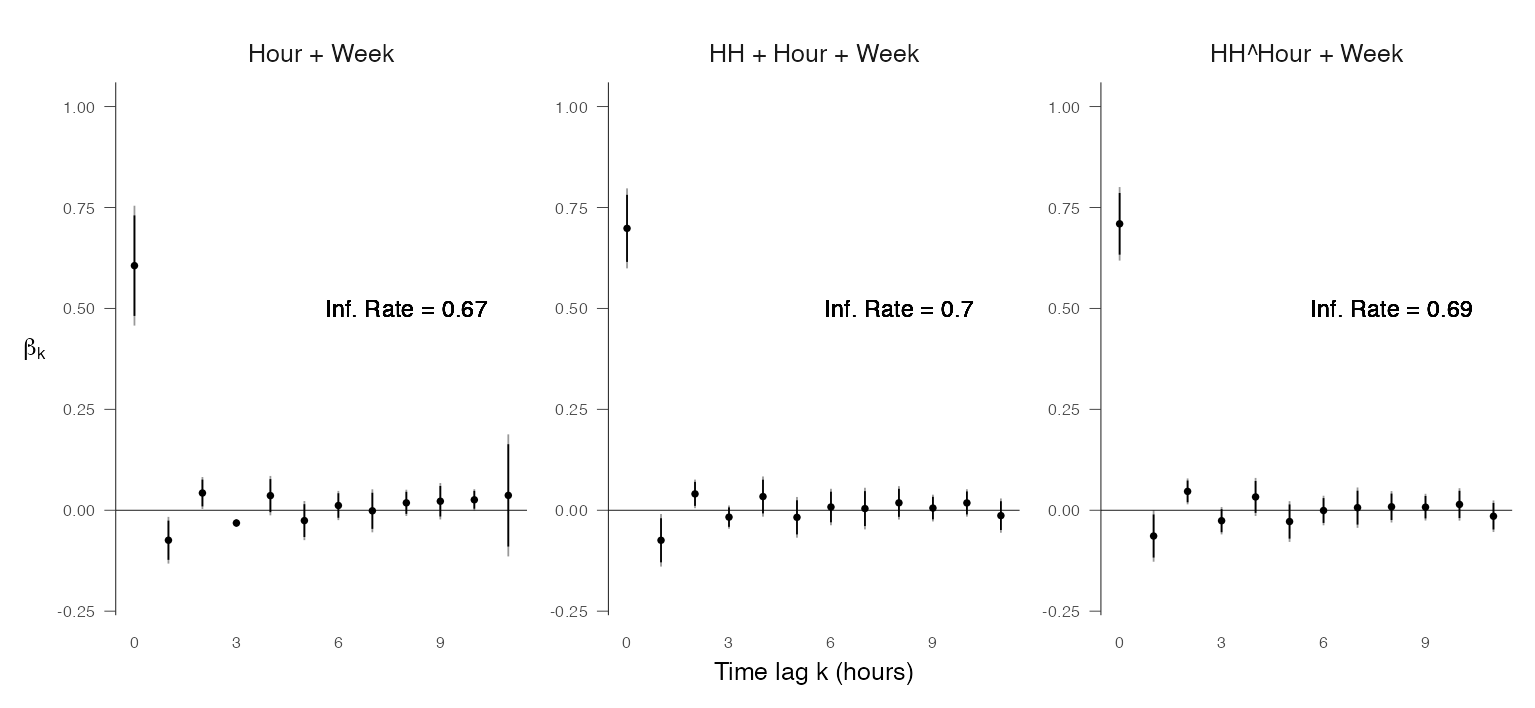
\includegraphics[width=.9\linewidth]{output_clean/figures/inf_lags.png}
    \caption*{\footnotesize Notes: Infiltration rate, showing the relationship between changes in outdoor concentration and changes in indoor concentrations. This shows the lags in the previous 11 hours. The model controls for ontrols for hyperlocal source variables (waste burning frequency, household smoking, kitchen source presence, cooking activity, and distance to main road), outdoor temperature, humidity, and hour-of-day and week fixed effects. Points represent mean estimates; darker error bars show 90\% confidence intervals, and lighter error bars show 95\% confidence intervals. Errors are clustered at the household level. }
    \label{fig:inf_lag}
\end{figure}

\begin{figure}[!htb]
    \centering
    \caption{Robustness: Mean $PM_{2.5}$ Under Various Aggregation Methods} 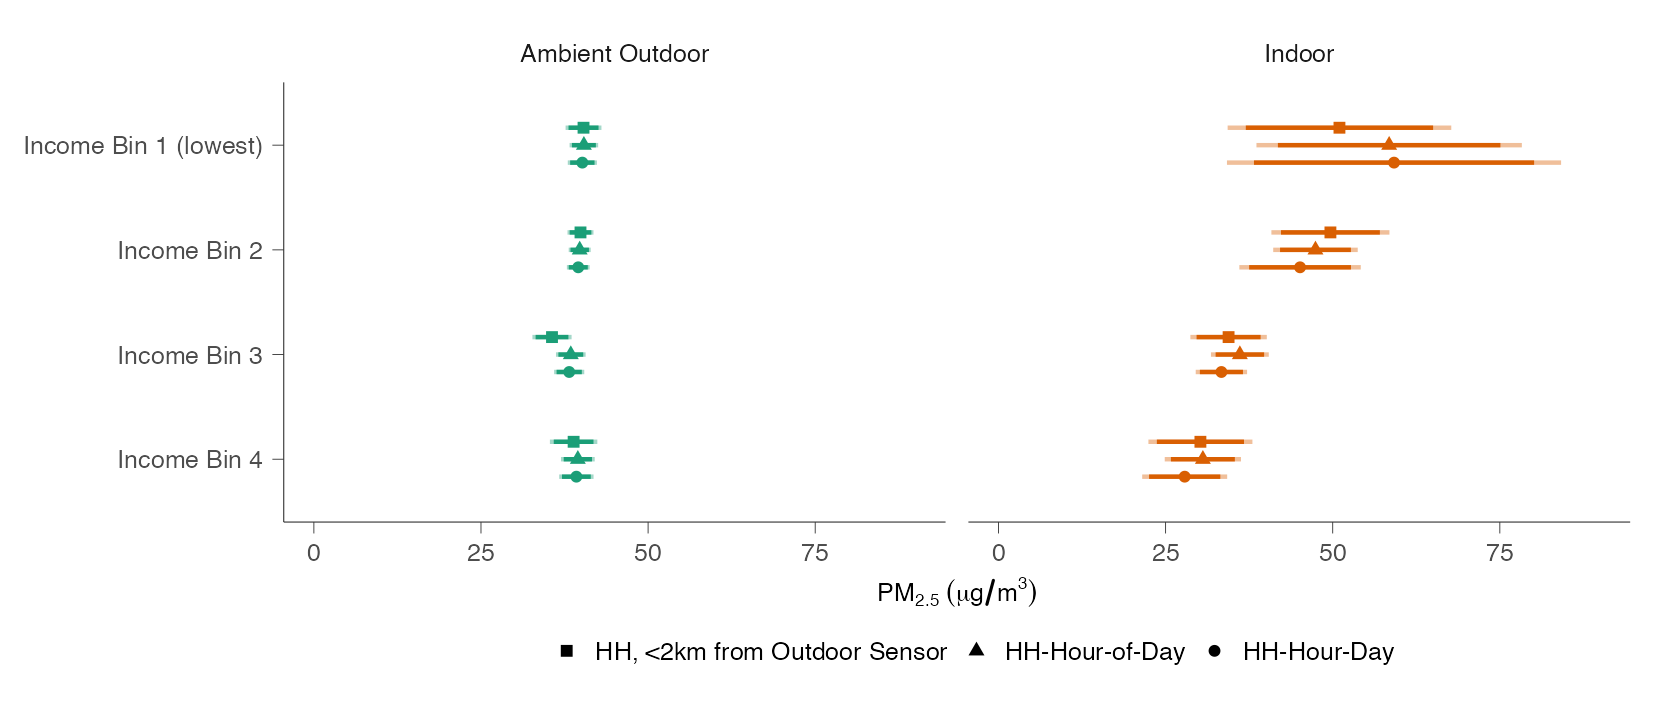
\includegraphics[width=\linewidth]{output_clean/figures/pm_income_robustness.png}
    \caption*{\footnotesize Notes: \textbf{(a)} Mean $PM_{2.5}$ concentrations across income quartiles, aggregated using three different methods to show robustness. \textit{HH, $<2$km from Outdoor Sensor}, calculates a single mean \( PM_{2.5} \) value per household, restricting the sample to households located within 2 km of an outdoor sensor to ensure proximity-based comparability. \textit{HH-Hour-of-Day}, aggregates data by computing the mean \( PM_{2.5} \) concentration for each household at each hour of the day. \textit{HH-Hour-Day} uses mean \( PM_{2.5} \) concentrations at the level of each household-hour-date. These mean $PM_{2.5}$ is then regressed onto the income quartile. Points represent mean estimates; darker error bars show 90\% confidence intervals, and lighter error bars show 95\% confidence intervals. Errors are clustered at the household level.
 }
    \label{fig:pm_income_robust}
\end{figure}



\begin{figure}[!htb]
    \centering
    \caption{Spatial Correlation of Outdoor Sensor Pairs} 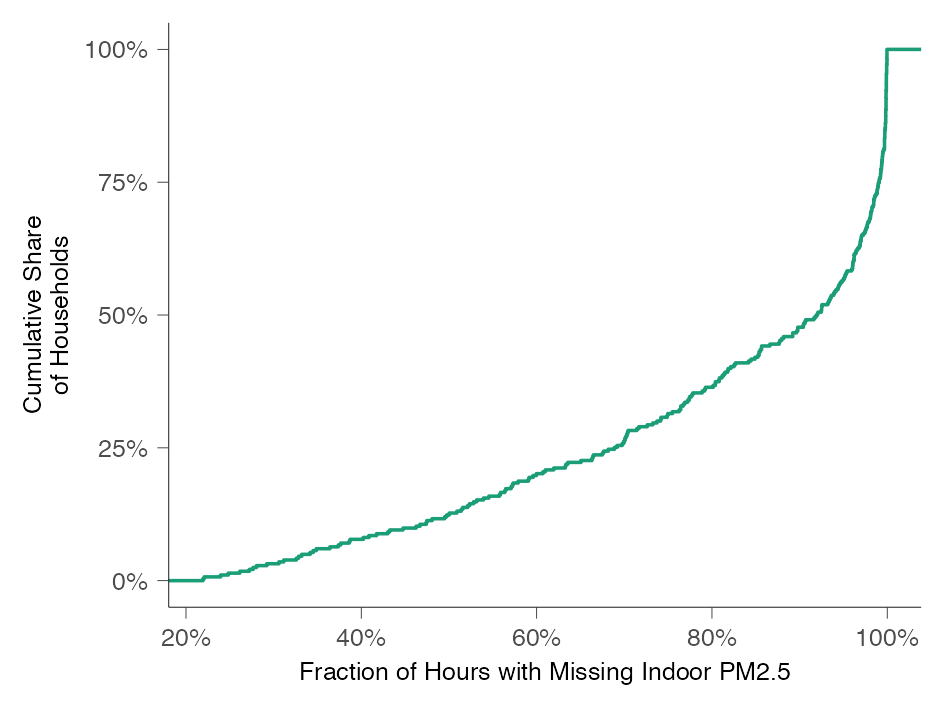
\includegraphics[width=.9\linewidth]{output_clean/figures/fig_appendix_missing_data.png}
    \caption*{\footnotesize Notes: Empirical cumulative distribution function of missing indoor PM$_{2.5}$ data. Each observation represents a household; the x-axis shows the fraction of that household's hourly PM$_{2.5}$ readings that are missing, and the y-axis shows the cumulative share of households at or below that fraction.}
    \label{fig:sensor_corelations}
\end{figure}


\clearpage
\section{Tables}
\setcounter{table}{0}
\renewcommand{\thetable}{A\arabic{table}}

\begin{table}[!h]
    \centering

    \resizebox{.7\textwidth}{!}{
    \begin{threeparttable}
    \caption{Summary Statistics of Household Survey}      \label{tab:covariates}
    
\begin{tabular}{lccc}
\toprule
Variable & Sample Mean & N & Population Mean\\
\midrule
Female & 0.9 & 283 & \\
 &  &  \vphantom{3} & \\
Age & 41.21 & 283 & \\
 & (6.91) &  & \\
HH Size & 5.13 & 283 & 3.79\\
 & (1.94) &  & (1.31)\\
Number of Children & 2.05 & 283 & \\
 & (1.03) &  & \\
HH Monthly Exp. (USD) & 248.74 & 275 & 655.94\\
 & (117.16) &  & (707.71)\\
HH Monthly Income (USD) & 312.48 & 281 & \\
 & (194.17) &  & \\
HH Head Attended Secondary & 0.88 & 283 & 0.88\\
 &  &  \vphantom{2} & \\
HH Head Attended Tertiary & 0.14 & 283 & 0.3\\
 &  &  \vphantom{1} & \\
Owns AC & 0.55 & 282 & 0.39\\
 & (0.5) &  & \\
LPG Stove & 0.98 & 283 & 0.96\\
 &  &  & \\
Number of Smokers & 0.93 & 283 & 0.73\\
 & (0.85) &  & (0.71)\\
\midrule
\bottomrule
\end{tabular}

    \begin{tablenotes}
      \footnotesize
      \item \textit{Notes:}  Household characteristics and comparisons to the Jakarta population mean. Population means were calculated using data from the National Socioeconomic Survey (SUSENAS) 2023.
    \end{tablenotes}
  \end{threeparttable}
    }
\end{table}



\begin{table}[!htb]

    \centering

    \resizebox{.7\textwidth}{!}{
    \begin{threeparttable}
    \caption{Distance to Outdoor Sensor Not Correlated with Household Characteristics}
    \label{tab:sensor_selection}

\begin{tabular}{lc}
   \toprule
   Dependent Variable:           & Distance to Outdoor Sensor (meters)\\  
   Model:                        & (1)\\  
   \midrule
   \emph{Variables}\\
   Indoor PM2.5                  & -0.99\\   
                                 & (2.44)\\   
   Outdoor PM2.5                 & 1.19\\   
                                 & (9.21)\\   
   Income (USD)                  & 0.13\\   
                                 & (0.58)\\   
   Housing Size                  & 42.52\\   
                                 & (53.36)\\   
   AC                            & -198.33\\   
                                 & (197.47)\\   
   HOH Employed                  & 314.69\\   
                                 & (374.62)\\   
   HOH Attended Secondary School & -285.71\\   
                                 & (305.55)\\   
   HOH Attended Tertiary School  & -173.15\\   
                                 & (317.86)\\   
   \midrule
   \emph{Fit statistics}\\
   Dependent variable mean       & 2,337.6\\  
   Observations                  & 283\\  
   \bottomrule
\end{tabular}



    \begin{tablenotes}
      \footnotesize
      \item \textit{Notes:} Regression of households' distance to nearest outdoor sensor on household covariates. IID standard-errors in parentheses. 
    \end{tablenotes}
  \end{threeparttable}
    }
\end{table}


\begin{table}[!h]
    \centering

    \resizebox{.7\textwidth}{!}{
    \begin{threeparttable}
    \caption{Summary Statistics of Household Survey}      \label{tab:covariates}
    
\begin{tabular}{cccccc}
\toprule
Source & Reg. Estimate & p.value & Mean Value of Source & Mean Contribution & $R^2$ Contribution\\
\midrule
Outdoor Ambient & 0.59 & 0.000 & 39.41 & 56\% & 33\%\\
Smoked (24 Hours) & 21.33 & 0.001 & 0.38 & 19\% & 23\%\\
Kitchen source & -0.28 & 0.968 & 0.31 & 0\% & 0\%\\
Cooking & -2.49 & 0.469 & 0.08 & 0\% & 0\%\\
Distance to Main Road (km) & 3.52 & 0.707 & 0.57 & 5\% & 0\%\\
\addlinespace
Waste Burning (1-2/week) & -1.76 & 0.743 & 0.21 & -1\% & \\
Waste Burning (3+/week) & 46.85 & 0.168 & 0.10 & 12\% & \\
\bottomrule
\end{tabular}

    \begin{tablenotes}
      \footnotesize
      \item \textit{Notes:}  Household characteristics and comparisons to the Jakarta population mean. Population means were calculated using data from the National Socioeconomic Survey (SUSENAS) 2023.
    \end{tablenotes}
  \end{threeparttable}
    }
\end{table}


\begin{table}[!h]
    \centering

    \resizebox{.7\textwidth}{!}{
    \begin{threeparttable}
    \caption{Summary Statistics of Household Survey}      \label{tab:covariates}
    
\begin{tabular}{cccccc}
\toprule
Source & Reg. Estimate & p.value & Mean Value of Source & Mean Contribution & $R^2$ Contribution\\
\midrule
Outdoor Ambient & 0.000 & 0.008 & 39.41 & 28\% & 2\%\\
Smoking Household & 0.032 & 0.000 & 0.38 & 57\% & 54\%\\
Kitchen source & -0.006 & 0.180 & 0.31 & -9\% & 2\%\\
Cooking & 0.008 & 0.191 & 0.08 & 3\% & 1\%\\
Distance to Main Road (km) & -0.006 & 0.109 & 0.57 & -16\% & 5\%\\
\addlinespace
Waste Burning (1-2/week) & -0.002 & 0.663 & 0.21 & -2\% & \\
Waste Burning (3+/week) & 0.047 & 0.164 & 0.10 & 23\% & \\
 &  &  &  &  & 19\%\\
\bottomrule
\end{tabular}

    \begin{tablenotes}
      \footnotesize
      \item \textit{Notes:}  Household characteristics and comparisons to the Jakarta population mean. Population means were calculated using data from the National Socioeconomic Survey (SUSENAS) 2023.
    \end{tablenotes}
  \end{threeparttable}
    }
\end{table}



\begin{table}[!h]
    \centering

    \resizebox{.7\textwidth}{!}{
    \begin{threeparttable}
    \caption{Summary Statistics of Household Survey}      \label{tab:covariates}
    % -----------------------------------------------------------------------
% Auto-generated by table_boe.R -- do not edit by hand
% -----------------------------------------------------------------------

\begin{tabular*}{\linewidth}{@{\extracolsep{\fill}}lccccc}
\toprule
%---- Panel A -------------------------------------------------------
\multicolumn{6}{l}{\textbf{Panel A. Data inputs and derived parameters}} \\[2pt]
  & $C_{in}$
  & $C_{out}$
  & $\hat{F}_{inf}$
  & $a$
  & $S$
  \\
  & ($\mu$g\,m$^{-3}$)
  & ($\mu$g\,m$^{-3}$)
  &
  & (h$^{-1}$)
  & ($\mu$g\,m$^{-3}$\,h$^{-1}$)
  \\
\cmidrule(lr){2-3}\cmidrule(lr){4-4}\cmidrule(lr){5-6}
Income Bin 1, Non-smoking & 49.0 & 40.0 & 0.593 & 0.7 & 31.0 \\
Income Bin 1, Smoking & 57.3 & 40.5 & 0.593 & 0.7 & 41.0 \\
Income Bin 4, Non-smoking & 28.2 & 40.0 & 0.551 & 0.6 & 6.9 \\
Income Bin 4, Smoking & 36.8 & 38.4 & 0.551 & 0.6 & 17.4 \\
\midrule
%---- Panel B -------------------------------------------------------
\multicolumn{6}{l}{\textbf{Panel B. Counterfactual $\Delta C_{in}$ ($\mu$g\,m$^{-3}$)}} \\[2pt]
  &
  \multicolumn{2}{c}{Weatherization ($a \times 0.8$)}
  &
  \multicolumn{2}{c}{Reduced Particle Penetration ($P \times 0.8$)}
  & \\
\cmidrule(lr){2-3}\cmidrule(lr){4-5}
  & Central
  & Robust.~range\textsuperscript{(a)}
  & Central
  & Direction
  & \\
\cmidrule(lr){2-3}\cmidrule(lr){4-5}
Income Bin 1, Non-smoking & $+1.2$ & [$+1.2$,\;$+2.9$] & $-4.7$ & Always $\downarrow$ & \\
Income Bin 1, Smoking & $+2.3$ & [$+2.3$,\;$+4.3$] & $-4.8$ & Always $\downarrow$ & \\
Income Bin 4, Non-smoking & $-1.5$ & [$-1.5$,\;$-0.6$] & $-4.4$ & Always $\downarrow$ & \\
Income Bin 4, Smoking & $-0.2$ & [$-0.2$,\;$+1.0$] & $-4.2$ & Always $\downarrow$ & \\
\bottomrule
\end{tabular*}

    \begin{tablenotes}
      \footnotesize
      \item \textit{Notes:}  Household characteristics and comparisons to the Jakarta population mean. Population means were calculated using data from the National Socioeconomic Survey (SUSENAS) 2023.
    \end{tablenotes}
  \end{threeparttable}
    }
\end{table}



\clearpage
\newpage
\section{Survey Questions}
\begin{enumerate}
\item What was your household's total income in the past month (in IDR)? This includes cash transfers from the government \\ \textit{ Berapa penghasilan rumah tangga dalam sebulan terakhir? (dalam Rupiah)}
\begin{enumerate}
    \item $<$Rp 1.000.000
    \item Rp 1.000.000 - Rp 2.999.999
    \item Rp 3.000.000 - Rp 4.999.999
    \item Rp 5.000.000-Rp 7.999.999
    \item Rp 8.000.000 - Rp 9.999.999
    \item Rp 10.000.000 - Rp12.999.999
    \item $>$13.000.000
        \item Does not know \\ \textit{Tidak tahu}
        \item Refuse to answer \\ \textit{Menolak menjawab}
\end{enumerate}
\item How many rooms does this residence have?

[Enumerator: Count spaces as separate rooms only if they have a formal entrance, even if the door is a curtain. Do not count one room divided by curtains without a formal entrance as separate rooms. Family-owned shops attached to the residence and bathrooms should counts as rooms.] \\ \textit{Berapa banyak kamar yang dimiliki hunian ini? 
[Enumerator: ruangan dianggap terpisah jika ada tempat masuk, meskipun pintunya adalah kain. Jika tidak ada tempat masuk, meski terpisah oleh kain/gorden, jangan dihitung sebagai ruangan terpisah. Toko yang bersatu dengan rumah, kamar mandi, dihitung sebagai satu ruangan terpisah.}

    \item In the past 7 days, how do you think air quality was in your home, on the scale we mentioned earlier? \\ \textit{Dalam seminggu terakhir, berdasarkan skala yang sudah saya sebutkan tadi, menurut Ibu/Bapak seberapa baik kualitas udara di Jakarta?}

    \begin{enumerate}
        \item Good (green) \\ \textit{Baik (hijau)}
        \item Moderate (yellow) \\ \textit{Sedang (kuning)}
        \item Unhealthy for sensitive groups (orange) \\ \textit{Tidak sehat untuk kelompok rentan (oranye)}
        \item Unhealthy (red) \\ \textit{Tidak sehat (merah)}
        \item Very unhealthy (purple) \\ \textit{Sangat tidak sehat (ungu)}
        \item Hazardous (Brown) \\ \textit{Berbahaya (coklat)}
        \item Doesn't know \\ \textit{Tidak tahu}
    \end{enumerate}
    \item Is there an air conditioner in the house? \\ \textit{Apakah terdapat AC/pendingin udara di dalam rumah?}
    \begin{enumerate}
        \item No \\ \textit{Tidak}
        \item Yes, in room the hardware is in \\ \textit{Ya, di ruangan yang terdapat air purifier dan air monitor}
        \item Yes, in another room in the house \\ \textit{Ya, di ruangan lain}
    \end{enumerate}
    \item In the last 24 hours, did someone smoke inside your home?	\\ \textit{Dalam 24 jam terakhir, apakah seseorang merokok di dalam rumah Anda?}
    \begin{enumerate}
        \item Yes \\ \textit{Ya}
        \item No \\ \textit{Tidak}
         \item Does not know \\ \textit{Tidak tahu}
        \item Refuse to answer \\ \textit{Menolak menjawab}
    \end{enumerate}
    \item In the past 7 days, how many times did you see trash being burned in your neighborhood? \\ \textit{Dalam seminggu terakhir, berapa kali Ibu/Bapak melihat sampah dibakar di lingkungan Ibu/Bapak?}
    \begin{enumerate}
        \item Never \\ \textit{Tidak pernah} 
        \item 1 or 2 times \\ \textit{1-2 kali}
        \item 3 or more times \\ \textit{3 kali atau lebih}
        \item Does not know \\ \textit{Tidak tahu}
        \item Refuse to answer \\ \textit{Menolak menjawab}
    \end{enumerate}
    \item What is the main cooking fuel you use in your home? \\ \textit{Apa bahan bakar utama untuk memasak yang Ibu/Bapak gunakan di rumah?}
    \begin{enumerate}
        \item Electric \\ \textit{Kompor listrik}
        \item Gas/LPG \\ \textit{LPG}
        \item Kerosene \\ \textit{Minyak tanah}
        \item Charcoal/briquettes/coconut shells \\ \textit{Arang/briket/batok kelapa}
        \item Firewood \\ \textit{Kayu bakar}
        \item Other \\ \textit{Lainnya}
    \end{enumerate}
    \item I have a list of activities that could cause air pollution in the room the hardware is set up in. Can you verify if any of the following occur in the room of the purifier? \\ \textit{Saya memiliki daftar aktivitas yang dapat menyebabkan polusi udara di ruangan tempat alat dipasang. Bisakah Ibu/Bapak memberitahu apakah terdapat aktivitas berikut yang terjadi di ruangan yang terdapat air purifier?}	
    \begin{enumerate}
        \item Gaps in doors and windows \\ \textit{Celah di pintu dan udara}
        \item Doors/windows are always open \\ \textit{Pintu/jendela yang selalu terbuka}
        \item Close to kitchen \\ \textit{Dekat dengan dapur} 
        \item Smoking/vaping in or near the room \\ \textit{Merokok/vaping di dalam/dekat ruangan}
        \item Whether the room has doors and is connected to another room \\ \textit{Ruangan memiliki pintu yang terhubung dengan ruangan lain}
        \item Garbage burning in the neighborhood \\ \textit{Pembakaran sampah di lingkungan sekitar}
        \item Candles/Incense \\ \textit{Difuser/Pelembab udara/humidifier}
        \item None
    \end{enumerate}

    
\end{enumerate}

We also asked households, via WhatsApp, about their window/door opening activities:
\begin{enumerate}
    \item In the last hour, was the door to the room where the air quality equipment is stored open to the outside? \\ \textit{Dalam 1 jam terakhir, apakah pintu di ruangan tempat menyimpan alat kualitas udara terbuka ke luar? (jika ada pintu yang terbuka ke luar ruangan)}
    \begin{enumerate}
        \item Yes \\ \textit{Ya}
        \item No \\ \textit{Tidak}
        \item There are no outside doors \\ \textit{Tiada pintu ke luar}
    \end{enumerate}
        \item In the last hour, was the window in the room where the air quality equipment is stored open to the outside? \\ \textit{Dalam 1 jam terakhir, apakah jendela di ruangan tempat menyimpan alat kualitas udara terbuka ke luar? (jika ada jendela yang terbuka ke luar ruangan)}
    \begin{enumerate}
        \item Yes \\ \textit{Ya}
        \item No \\ \textit{Tidak}
        \item There are no outside windows \\ \textit{Tak ada jendela luar}
    \end{enumerate}
\end{enumerate}

\end{document}